\section{Refinando petr\'oleo}
\subsection{Descripci\'on de la problem\'atica}
\subsection{Resoluci\'on propuesta y justificaci\'on}
\subsection{An\'alisis de la complejidad}
\subsection{C\'odigo fuente}
\subsection{Experimentaci\'on}
\subsubsection{Constrastaci\'on Emp\'irica de la complejidad}
	Para llevar a cabo esta experimentaci\'on, consideramos el peor caso posible de cantidad de ejes del grafo, es decir que habr\'a exactamente $n.(n-1)$ ejes (cada nodo puede conectarse con cualquier nodo del grafo, excepto consigo mismo), variando la cantidad de nodos.
	
	Los tiempos de ejecuci\'on para cada n (cantidad de nodos) fueron los siguientes:
	
	\begin{table}[htb]
	\centering
	\begin{tabular}[c]{|l|l|}

		\hline
n & Tiempo en segundos\\
		\hline
50	&	0.0005254864\\
		\hline
100	&	0.002332719\\
		\hline
150	&	0.0059328642\\
		\hline
200	&	0.01065945\\
		\hline
250	&	0.0178728144\\
		\hline
300	&	0.0277215188\\
		\hline
350	&	0.0373807766\\
		\hline
400	&	0.0487278266\\
		\hline
450	&	0.0661190683\\
		\hline
500	&	0.0807527896\\
		\hline
550	&	0.0978193478\\
		\hline
600	&	0.126140013\\
		\hline
650	&	0.146378511\\
		\hline
700	&	0.168847877\\
		\hline
750	&	0.192539493\\
		\hline
800	&	0.219705288\\
		\hline
850	&	0.267457097\\
		\hline
900	&	0.301437881\\
		\hline
950	&	0.332602623\\
		\hline
1000	&	0.366929358\\
		\hline
		
	\end{tabular}
	%\caption{Tabla muy sencilla.}
	%\label{tabla:n.png}
	\end{table}

  \begin{figure}[h!]
   \begin{center}
 	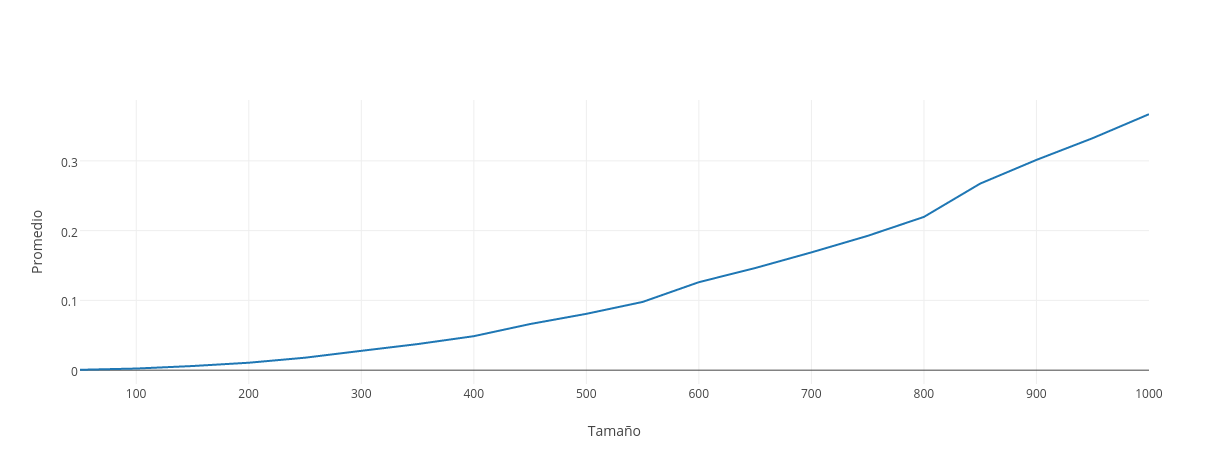
\includegraphics[scale=0.4]{imagenes/ej3/n2logn.png}
% 	\caption{}
% 	\label{n.png}
   \end{center}
 \end{figure}
 \newpage

Dado que la Cota de Complejidad planteada te\'oricamente es de $O(n^2.log(n))$, era esperable que la curva sea una par\'abola creciente.

A simple vista, no se puede apreciar si la relaci\'on que tienen respecto de tama\~no/tiempo es efectivamente la que buscamos (pues casi todas las curvas polinomiales tienen gr\'aficos similares). Por este motivo, como siguiente paso decidimos comenzar a linealizar los tiempos, dividiendo a cada uno por $log(n)$.

   \begin{figure}[h!]
   \begin{center}
 	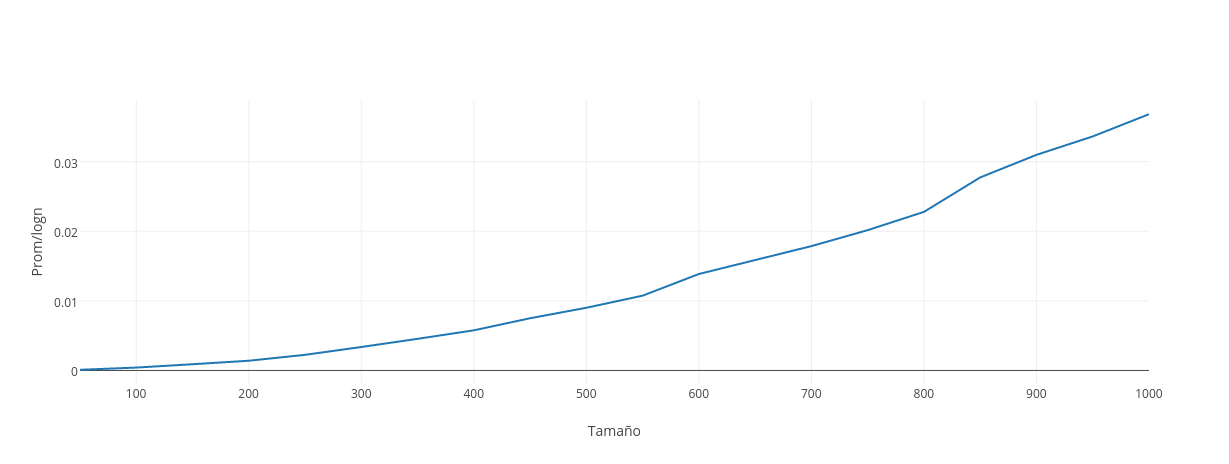
\includegraphics[scale=0.4]{imagenes/ej3/n2.png}
% 	\caption{}
% 	\label{caballito}	
   \end{center}
 \end{figure}
 \newpage

	La morfolog\'ia de este gr\'afico es similar a la anterior, sigue siendo una par\'abola creciente, por lo tanto terminaremos de linealizar, dividiendo a cada uno por $n$, para ver si se trata de la par\'abola cuadr\'atica.\\

   \begin{figure}[h!]
   \begin{center}
 	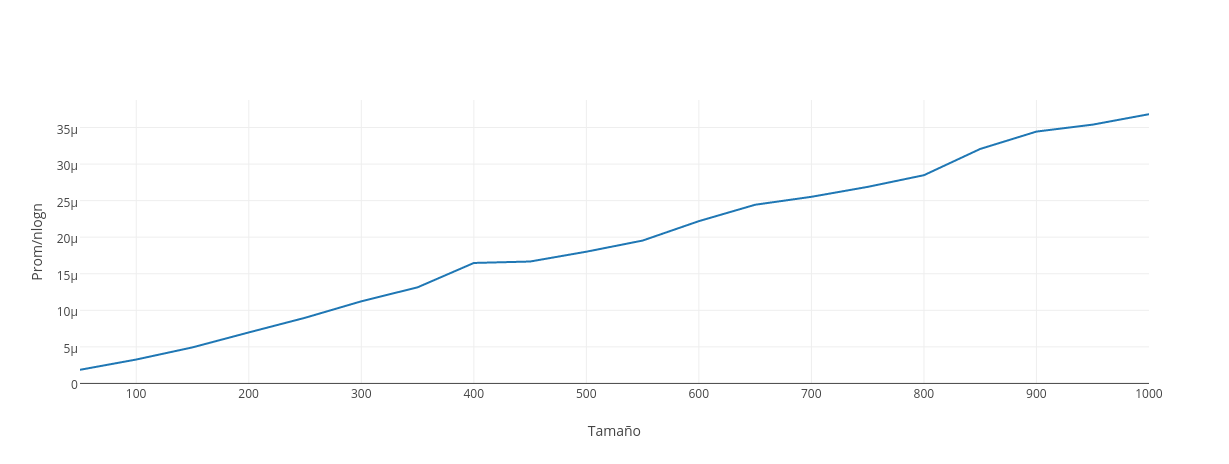
\includegraphics[scale=0.4]{imagenes/ej3/n.png}
% 	\caption{}
% 	\label{caballito}	
   \end{center}
 \end{figure}
 \newpage

	Efectivamente puede observarse que el comportamiento es lineal. Por lo tanto, podemos afirmar que nuestra experimentaci\'on condice a la Cota Te\'orica planteada de $O(n^2.log(n))$.